\documentclass{report}

%packages
\usepackage{graphicx}
\usepackage{url}
\usepackage{amsmath}

% title stuff
\author{Martin Knudsen}
\title{The Error Function - Latex trial document for Practical Programming 2018}


\begin{document}
\maketitle

\section*{Introduction}
The error function is a particular important function that occurs in many areas of mathematics including probability theory and statistics. It is defined as in equation\eqref{eq:error}.\cite{wiki} 

\begin{equation}
u(x) = \frac{1}{\sqrt{\pi}}\int ^x_{-x}e^{-t^2}\mathrm{d}t
\label{eq:error}
\end{equation} 

and looks like figure \ref{fig:error}. 

The meaning of the error function in statistics is that for a random normally distributed variable \textit{Y} which has mean 0 and variance 1/2 \eqref{eq:error} describes the probability of \textit{Y} falling in the range $[-x,x]$. \cite{wiki}. 

\begin{figure}[tbph]
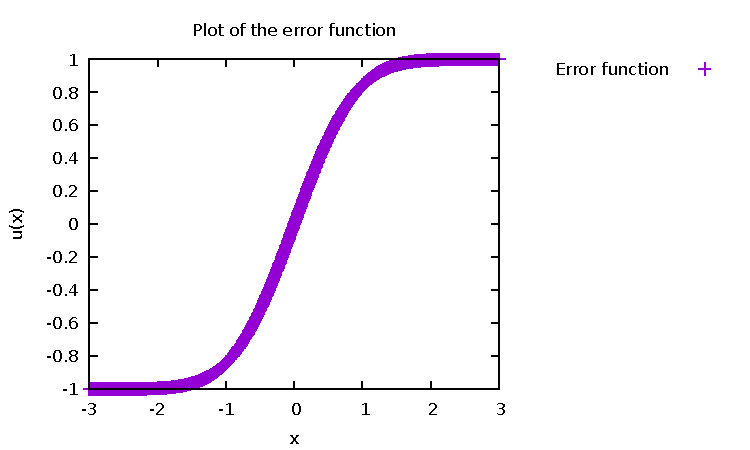
\includegraphics[width=1.0\textwidth]{error_function_plot}
\caption{Plot of the Error function as a function of the argument x. Found using the odeiv2 environment of GSL. \label{fig:error}}
\end{figure}

\subsection*{Properties}
It has some interesting properties such as being an odd function $u(-x)=-u(x)$ and that the complex conjugate of the function is a equal to the function of the complex conjugate of the argument $u(\overline{x})=\overline{u(x)}$.\cite{wiki}

\section*{Applications}
When measurements are descibed by a normal distribution with standard deviation $\sigma$ and expectation value 0 then $u\Big(\frac{a}{\sigma\sqrt{2}}\Big)$ is the probsbility that a measurement will lie in the interval $[-a, a]$\cite{wiki}. One can see that this is coherent with the definition above when $\sigma=1/2$. An example of such a situation is when detecting scattered particles in Rutherford scattering. The energy of the scattered particles are normally distributed and hence the error function can be used (if $\sigma$ is known) to determine the properbility to measure energy outside a certain interval around the mean. 

% begin bibliography just normal one. 
\bgroup
\let\clearpage\relax
\begin{thebibliography}{9}

\bibitem{wiki}
Wikipedia contributors, 
(02.27.2018) Error function, Retrieved 12.03.2018, 
from \url{https://en.wikipedia.org/wiki/Error_function}.

\end{thebibliography}
\egroup

\end{document}